\documentclass[../main.tex]{subfiles}
\begin{document} \label{chapter_account}
In this chapter, we describe our implementation of the general pipeline described in section \ref{general_pipeline} and the achieved results. On one hand, we describe the birdsong dataset and the corresponding preprocessing techniques we used, as well the algorithms and packages used to implement formant trajectory extraction, Kernel Density Estimation, Variational Hidden Markov Models and Agglomerative Hierarchical Clustering, as described in chapters \ref{chapter_formants} and \ref{chapter_hmms}. On the other hand, we present the achieved relational structures (henceforth called phylo-acoustic trees) and other experiments performed over birdsong data.

\section{Implementation}
We implemented a system capable of building phylo-acoustic trees automatically. The implementation runs in MATLAB 2015a and all the experiments were executed on a computer with an Intel i5-3317U CPU, 8.00 GB RAM, running Windows 8.1 64-bits. 
\par With respect to the data, we used the Animal Sound Archive bird vocalisation dataset, which contains 3686 birdsong recordings of more than 100 different bird species from all over Europe. We used the data for 82 bird species that had at least 15 seconds of birdsong recording each. All the recordings are in WAV format (i.e. uncompressed) and sampled at 22,500 Hz, for reasons that will become clearer when we present the formant trajectory extraction implementation. 

\section{Formant trajectory extraction} \label{section_impformants}
As reviewed in chapter \ref{chapter_formants}, the goal of formant trajectory extraction is to generate a vector $\V{F} = \{\V{f}_1, \V{f}_2, ..., \V{f}_W\}$ of formants $\V{f}_i$ in each window. We now use the signal processing techniques described in section \ref{subsection_preproc}: a pre-emphasis filtering with $\alpha = 0.95$ is first applied to the birdsong recording, which is then segmented into frames of 40 ms with an overlap of 50\% \cite{Stowell2014}. Every frame is then convoluted with a Hamming window to avoid sharp-edged frames. 
\par The number of formants we estimate per window corresponds to the rule of thumb $N_f = f_s / 2000$, where $f_s$ is the sampling frequency of the recording. Since birdsong goes to frequencies as high as 10,000 Hz \cite{Marler2004}, and that we want to have 1 formant per thousand Hz, all the birdsong files must be sampled at 22,500 Hz. Furthermore, the order of the LPC model corresponds to the rule of thumb $p = 2N_f + 2$, i.e. we have 1 formant for every 2 roots, and let the model have an extra 2 roots to handle very low frequencies where large amounts of energy are contained, but are not resonances of the vocal tract \cite{Benesty}. 
\par Finally, the autocorrelation $\V{r}$ is estimated by using the Wiener-Khinchin Theorem and the rest of the formant trajectory extraction proceeds as outlined in chapter \ref{chapter_formants}, and summarised in algorithm \ref{alg_formants}. MATLAB contains an implementation of the Fast Fourier Transform algorithm and polynomial root solving algorithms. Furthermore, the Signal Processing Toolbox contains an implementation of the Levinson-Durbin recursion. These algorithms were assembled in a single, parametrised procedure to extract formants from recordings.

\begin{algorithm}
\begin{algorithmic}[1]
\Function{formants}{$\V{s}_i$, $f_s$, $N_f$}
\State $\V{S}$ = fft($\V{s}$)
\State $\V{R}$ = inv\_fft( $\V{S} \cdot \bar{\V{S}}$ )
\State $\V{a}$ = levinson($\V{r}, p$)
\State $\left[\V{r}, \theta\right]$ = roots($\V{a}$)
\State $\V{f}_i$ = $\theta \cdot \frac{f_s}{2\pi}$
\State $\V{b}_i$ = $-\frac{f_s}{4\pi}\log{\V{r}}$
\EndFunction
\caption{Formant extraction for a signal $\V{s}$.}\label{alg_formants}
\end{algorithmic}
\end{algorithm}

\par Once the formants for a given window have been calculated, all values $f_{i, j} < 500 Hz$ are filtered as noise \cite{Stowell2014}, and only the formants with a bandwidth narrower than 500 Hz are kept \cite{Mathworks2015}. Now, define $\bar{f}_k$ as:
\begin{align*}
\bar{f}_k = \sum_{i=1}^{W-1} \abs{f_{i+1, k} - f_{i,k}}
\end{align*}
\par In section \ref{section_choosing}, we show that the dataset exhibits a clear tendency of having $\bar{f}_1 < \bar{f}_{k'}, k'>1$. This suggests that by keeping only the first formant, we are keeping the smoothest trajectory of each recording. Figure \ref{fig_traj} depicts the first formant trajectory extracted from a birdsong recording of the species \emph{Certhia brachydactyla}.

\begin{figure}[t]
\centering
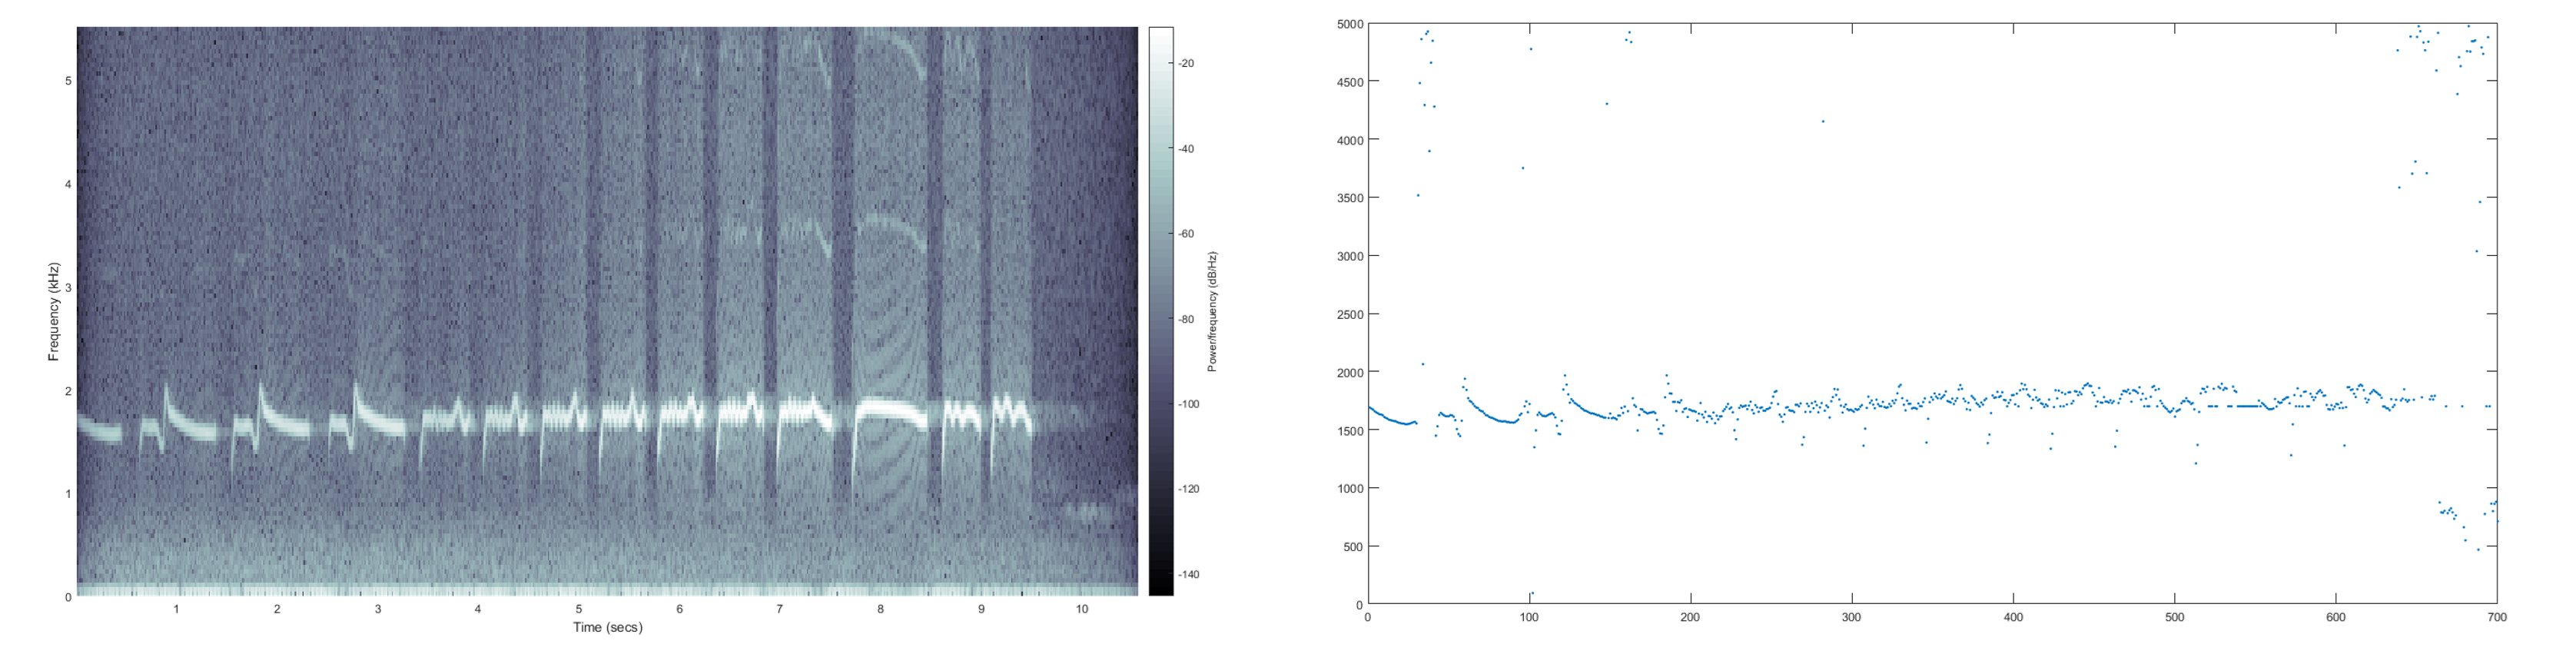
\includegraphics[width=\textwidth]{formant_traj}
\caption{To the right, the first formant trajectory extracted from a birdsong recording of the species \emph{Certhia brachydactyla}; to the left, the spectrogram corresponding to this recording. Note that the extracted trajectory corresponds with the bright patterns in the spectrogram, where present.}
\label{fig_traj}
\end{figure}

\section{Kernel Density Estimation and Hidden Markov Models} \label{section_imphmms}
In this section, we describe de implementations of Kernel Density Estimation and Variational Hidden Markov Models.
\par The function ksdensity is included in the MATLAB Statistics and Machine Learning Toolbox. It receives as input a vector of formants $\V{x}$ and an interval of points $\V{p}$ to evaluate the probability distribution at. For the case of univariate Gaussian kernels, it sets the bandwidth $h$ to a theoretical optimal, as discussed in section \ref{section_kde}. After estimating the probability distribution of each recording, all the distributions corresponding to the same species are averaged to obtain a single, characterising distribution per species. Figure \ref{fig_kdespecies} shows the result of this procedure for 5 different bird species in the ASA dataset.

\begin{figure}[t]
\centering
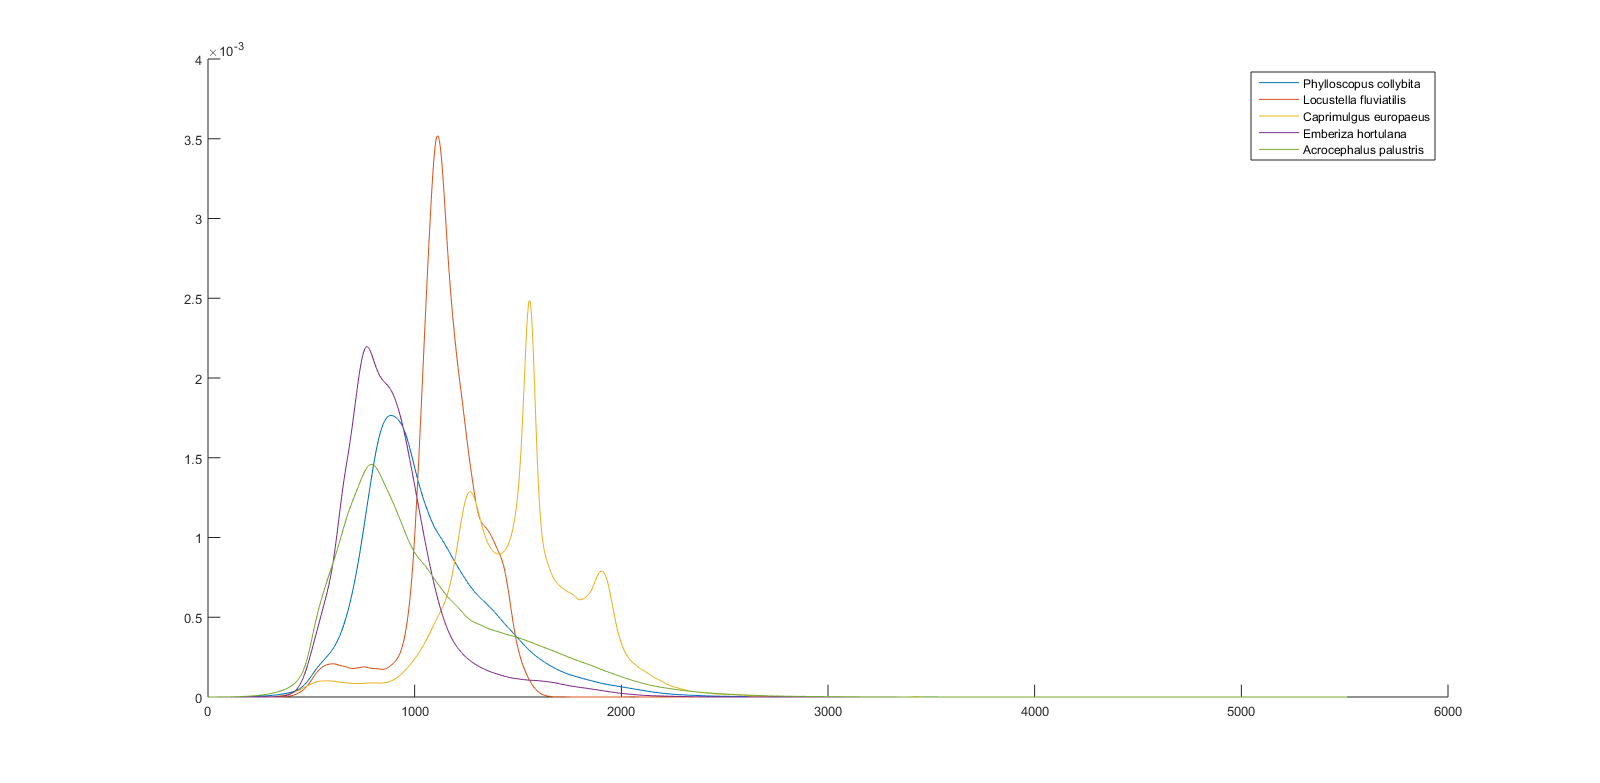
\includegraphics[width=\textwidth]{kdespecies}
\caption{Comparison of probability distributions generated by KDE for 5 different species. Despite having high probability in similar ranges of frequencies, their shapes are still distinguishable. }
\label{fig_kdespecies}
\end{figure}

\par Concerning Variational HMMs, we used the implementation of the Oxford Machine Learning Research Group, HMMBOX 4.1, which requires the NETLAB package. The former contains implementations of the tools required for a Bayesian treatment of HMMs, in particular: implementation of closed forms for the KL-divergence of the Normal, Dirichlet and Wishart distributions, variational inference training and sequence decoding. Furthermore, a routine that computes the occupancy of an HMM $\Omega_\lambda$ with respect to a sequence $\V{x}$ was also implemented. 
\par After computing the formant trajectories for each recording, the ones corresponding to a single species were concatenated and used as the training sequence for each HMM, i.e. we trained one HMM per species, and then computed their occupancy with respect to their respective training sequences. We used a Gaussian observation model for every HMM.

\section{Similarity matrices and Hierarchical Clustering}
The Hellinger distance and the Symmetric KL Divergence were implemented in MATLAB to compute distances between discrete distributions. These were used to compute the distance between each pair of densities obtained from the KDE procedure. In MATLAB, this can be done efficiently by means of the pdist function, a vectorised implementation that receives a metric and a matrix with observations as rows, and computes distance between each pair of rows.
\par With respect to HMMs, similarity computation is performed in two different approaches: one consists in computing the Hellinger distance or the SKLD between each pair of emission models (Gaussian Mixture Models). The other approach consists in sorting the HMMs' states (so as to avoid the identifiability problem discussed in chapter \ref{chapter_hmms}, and then computing the distance between each pair of Dirichlet distributions from the transition model. This distance metric corresponds to the definition given in equation \ref{eq:hmmdist}.
\par Then, we used the distance matrices obtained from these procedures to generate the phylo-acoustic tree using Agglomerative Hierarchical Clustering. The MATLAB Statistics and Machine Learning Toolbox contains routines to compute the three linkage procedures described in section \ref{section_hierarchical}. In particular, the function linkage receives a distance matrix and outputs a new matrix $\V{Z}$. The first two columns of $\V{Z}$ correspond to the identifiers of the merged clusters, and the third column displays the intergroup distance between the two clusters at time of merging. Additionally, the results of this stage can be evaluated by means of the cophenetic correlation coefficient, implemented in MATLAB via the cophenet function.
\par Finally, the dendrogram function was used to plot the clusters resulting from the linkage stage as a tree. Due to the monotonicity of agglomerative clustering, a dendrogram representation of the $\V{Z}$ is always available. 

\section{Conclusion} \label{section_5conclusion}
In this section, we described the implementation of the algorithms described in chapters  \ref{chapter_formants} and \ref{chapter_hmms}. A flowchart summarising these approaches is depicted in figure \ref{implementation_pipeline}. The results outcoming from each of these will be presented in chapter \ref{chapter_results}. 

\begin{figure}
\centering
\begin{tikzpicture}[node distance=2cm]
\node (start) [startstop] {Start};
\node (in1) [io, below of=start] {Animal Sound Archive dataset};
\node (pro1) [process, below of=in1] {Formant trajectory extraction};
\node (in2) [io, below of=pro1] {Formant trajectories};
\node (pro2) [process, below left=of in2] {KDE};
\node (pro2b) [process, below right=of in2] {Train HMM};
\node (pro3) [process, below = 2.5 cm of pro2] {Compute SKLD or Hellinger};
\node (pro3b) [process, below left=1 cm and -1.4 cm of pro2b] {SKLD/Hellinger between GMMs};
\node (pro3c) [process, below right=1 cm and -1.4 cm of pro2b] {Distance between Dirichlets};
\node (pro4) [process, below=7cm of in2] {Build relational structure};
\node (out1) [io, below=of pro4] {Relational structure};
\draw [arrow] (start) -- (in1);
\draw [arrow] (in1) -- (pro1);
\draw [arrow] (pro1) -- (in2);
\draw [arrow] (in2) -- (pro2);
\draw [arrow] (in2) -- (pro2b);
\draw [arrow] (pro2) -- (pro3);
\draw [arrow] (pro2b) -- (pro3b);
\draw [arrow] (pro2b) -- (pro3c);
\draw [arrow] (pro3) -- (pro4);
\draw [arrow] (pro3b) -- (pro4);
\draw [arrow] (pro3c) -- (pro4);
\draw [arrow] (pro4) -- (out1);
\end{tikzpicture}
\caption{A general pipeline to build relational structures.}
\label{implementation_pipeline}
\end{figure}



\end{document}